%==============================================================================
%  MATH 231 -- Linear Algebra I (Queens College, Fall 2026)
%  VECTOR UNIT, PART 5 -- Orthogonality, Independence, and Subspaces
%
%  This is one of the documents covering the vector unit. Section numbering
%  runs CONTINUOUSLY across all parts, so that every cross-reference in the
%  unit means the same thing no matter which part it appears in:
%
%      Part 1  MATH231_vectors_1_definition_and_arithmetic  Sections 1-9
%      Part 2  MATH231_vectors_2_dot_product_and_projection Sections 10-12
%      Part 3  MATH231_vectors_3_norms_and_metrics          Sections 13-15
%      Part 4  MATH231_vectors_4_basis_and_span             Sections 16-20
%      Part 5  MATH231_vectors_5_orthogonality_and_subspaces Sections 21-24
%
%  Hence the \setcounter{section}{20} below: this part opens at Section 21.
%
%  STATUS: complete.  Sections 21-24.  Sec. 24 closes the unit by restating
%  every definition in R^n with Sigma notation, so it is the reference section
%  students should return to.
%
%  AUDIENCE: distributed to students.  Keep it free of instructor-facing
%  apparatus -- time budgets, pacing notes, teaching cues.
%
%  TWO PRECISIONS against the drafted outline, both deliberate:
%
%   (a) The lemma needs the vectors to be NONZERO.  The zero vector is
%       orthogonal to everything, so {0, v} is vacuously "mutually orthogonal"
%       yet dependent and spans only a line.  Sec. 21.3 states the hypothesis.
%
%   (b) "Mutually orthogonal vectors in R^3 span R^3" needs THREE of them, and
%       its proof needs "three independent vectors in R^3 span R^3" -- the
%       general form of Sec. 18.5, which was proved only for n = 2.  Sec. 21.4
%       proves the independence half in full and flags the spanning half as
%       owed, rather than passing it off as done.
%
%  Sec. 21.1 finally states linearity of the dot product.  It was not needed
%  before -- Sec. 12.6 was done in components on purpose -- but the proof in
%  21.2 is the one that survives into R^n, and it needs it.
%
%  Compile with pdflatex (standard TeX Live packages only; uses tikz).
%==============================================================================
\documentclass[11pt]{article}

\usepackage[margin=1in]{geometry}
\usepackage{amsmath,amssymb,amsthm}
\usepackage[dvipsnames]{xcolor}
\usepackage{enumitem}
\usepackage{booktabs}
\usepackage{array}
\usepackage[hidelinks]{hyperref}
\usepackage{titlesec}
\usepackage{needspace}
\usepackage{tikz}
\usetikzlibrary{arrows.meta}

%------------------------------------------------------------------ style ----
\titleformat{\section}{\large\bfseries\sffamily}{\thesection.}{0.6em}{}
\titleformat{\subsection}{\normalsize\bfseries\sffamily}{\thesubsection.}{0.5em}{}
\titlespacing*{\section}{0pt}{14pt}{6pt}

\theoremstyle{definition}
\newtheorem{defn}{Definition}[section]
\newtheorem{ex}{Example}[section]
\theoremstyle{remark}
\newtheorem*{rmk}{Remark}
\newtheorem*{warn}{A common confusion}

\newcommand{\lookahead}{\par\smallskip\noindent
  \textbf{\sffamily\textcolor{RoyalBlue}{Looking ahead.}}\ \ignorespaces}

%--------------------------------------------------------------- notation ----
\newcommand{\R}{\mathbb{R}}
\newcommand{\Sph}[1]{\mathbb{S}^{#1}}
\newcommand{\vc}[1]{\mathbf{#1}}
\newcommand{\norm}[1]{\lVert #1\rVert}
\newcommand{\uv}[1]{\hat{\vc{#1}}}
\newcommand{\proj}[2]{\operatorname{proj}_{#1}(#2)}
\newcommand{\comp}[2]{\operatorname{comp}_{#1}(#2)}
\newcommand{\ivec}{\vec{\imath}}
\newcommand{\jvec}{\vec{\jmath}}
\newcommand{\kvec}{\vec{k}}
\newcommand{\bas}{\mathcal{B}}
\DeclareMathOperator{\spanop}{span}

%------------------------------------------------------------- tikz helpers --
\tikzset{
  vecarr/.style   = {-{Stealth[length=2.6mm,width=2.0mm]},very thick},
  thinarr/.style  = {-{Stealth[length=2.2mm,width=1.7mm]},thick},
  axisline/.style = {->,gray!75,thin}
}
\newcommand{\lattice}[4]{%
  \draw[step=1cm,gray!25,very thin] (#1,#3) grid (#2,#4);
  \draw[axisline] (#1,0) -- (#2+0.45,0) node[right,font=\scriptsize,black]{$x$};
  \draw[axisline] (0,#3) -- (0,#4+0.45) node[above,font=\scriptsize,black]{$y$};
}

\title{\vspace{-1.2cm}\textbf{\sffamily MATH 231 -- Linear Algebra I}\\[4pt]
       {\large\sffamily The Vector Unit, Part 5 \textbullet\ Orthogonality,
        Independence, and Subspaces}\\[2pt]
       {\normalsize\sffamily Kiely Hall 326 \textbullet\
        Instructor: Kevin Bedoya}}
\author{}
\date{}

\begin{document}
\setcounter{section}{20}  % this part opens at Section 21; see the header note
\maketitle
\vspace{-1.6cm}

\noindent\textbf{About this document.} This is Part 5 of the vector unit.
Section numbering runs continuously through all parts, so a reference such as
\S18.5 points into Part 4 and means exactly what it says:

\begin{center}
\renewcommand{\arraystretch}{1.2}
\begin{tabular}{@{}l l l@{}}
\toprule
\textbf{Part} & \textbf{Sections} & \textbf{Subject} \\
\midrule
1 & \S1--\S9    & vectors, notation, addition, scaling, equality \\
2 & \S10--\S12  & orientation, the dot product, projection \\
3 & \S13--\S15  & Cauchy--Schwarz, metrics, norms \\
4 & \S16--\S20  & the standard basis, span, coordinates, $\R^{3}$ \\
5 & \S21--\S24  & orthogonality, independence, subspaces, $\R^{n}$ \\
\bottomrule
\end{tabular}
\end{center}

\noindent\textbf{Assumed from Parts 1--4.} The dot product and the
orthogonality test $\langle\vc{u},\vc{v}\rangle=0$ (\S11.7); the identity
$\langle\vc{u},\vc{u}\rangle=\norm{\vc{u}}^{2}$ (\S11.6); projections (\S12.4);
span, basis, coordinates and dimension (\S16--\S17); linear independence
(\S18.4) and the fact that an independent pair spans $\R^{2}$ (\S18.5);
subspaces (\S19).

\medskip
\noindent\textbf{What you should be able to do afterwards.} State and use
linearity of the dot product; prove that mutually orthogonal nonzero vectors are
linearly independent, both geometrically and algebraically; state the lemma that
such vectors span; explain why the converse fails; compute coordinates against
an orthogonal basis by projection alone; describe the subspaces of $\R^{2}$
and $\R^{3}$ as lines and planes through the origin; prove the Pythagorean
identity and use it to account exactly for a projection; and state every
definition of the unit in $\R^{n}$ using $\Sigma$ notation.

%==============================================================================
\section{Orthogonality and independence}
%==============================================================================
Part 4 asked which pairs of vectors form a basis and answered: the independent
ones. But independence is a slightly awkward condition to check --- you set up a
combination equal to $\vc{0}$ and solve a system. This section shows there is a
sufficient condition that is far easier to test, one we have had since \S11.7.

%------------------------------------------------------------------------------
\subsection{What we will use: the dot product is bilinear}
%------------------------------------------------------------------------------
Until now most dot-product computations have been done by expanding into
coordinates; \S12.6 verified an orthogonality claim that way on purpose. The
argument in \S21.2 is different, because it is the one that keeps working in
dimensions we cannot draw, and instead of coordinates it uses the algebraic laws
collected in \S11.8. The piece it needs is bilinearity, in this combined form:
\[
  \bigl\langle \vc{u},\ \alpha\vc{v}+\beta\vc{w}\bigr\rangle
  = \alpha\langle\vc{u},\vc{v}\rangle + \beta\langle\vc{u},\vc{w}\rangle ,
\]
which is \textbf{D2} and \textbf{D3} applied together, and which by symmetry
(\textbf{D1}) holds in the first argument as well. Recall also \textbf{D4},
$\langle\vc{u},\vc{u}\rangle=\norm{\vc{u}}^{2}$.

Worth noting once: none of the verifications in \S11.8 mentioned how many
coordinates a vector has, so every one of \textbf{D1}--\textbf{D4} holds verbatim
in $\R^{3}$ and in $\R^{n}$. That is what makes the argument below
dimension-independent, and it is why we reach for the laws rather than the
components.

%------------------------------------------------------------------------------
\subsection{Orthogonal vectors are independent}
%------------------------------------------------------------------------------
\begin{quote}
\textbf{Claim.} If $\vc{u}$ and $\vc{v}$ are nonzero and orthogonal, then they
are linearly independent.
\end{quote}

\subsubsection*{The intuition}
Take the geometric route first, because it is a single sentence. Two nonzero
vectors are dependent exactly when they are parallel (\S18.4), and parallel
means the angle between them is $\theta=0$ or $\theta=\pi$. Orthogonal means
$\theta=\pi/2$. A pair cannot have two different angles, so an orthogonal pair
cannot be a parallel pair, and therefore cannot be dependent.

Put less formally: dependence means one vector is a stretched copy of the other,
so it lies entirely \emph{along} it. Orthogonal vectors lie entirely
\emph{across} each other --- neither has any component in the other's direction
at all, which is what a zero dot product says. Stretching something that points
due east will never produce something pointing due north.

\subsubsection*{The proof that survives into higher dimensions}
The geometric argument leans on $\theta$, which is a picture. Here is the same
fact without one. Suppose
\[
  \alpha\vc{u} + \beta\vc{v} = \vc{0} .
\]
Take the dot product of both sides with $\vc{u}$. The right side gives
$\langle\vc{u},\vc{0}\rangle=0$, and the left side expands by \S21.1:
\[
  \bigl\langle \vc{u},\ \alpha\vc{u}+\beta\vc{v}\bigr\rangle
  = \alpha\langle\vc{u},\vc{u}\rangle + \beta\langle\vc{u},\vc{v}\rangle
  = \alpha\norm{\vc{u}}^{2} + \beta\cdot 0
  = \alpha\norm{\vc{u}}^{2} ,
\]
using $\langle\vc{u},\vc{u}\rangle=\norm{\vc{u}}^{2}$ from \S11.6 and
orthogonality to kill the cross term. So $\alpha\norm{\vc{u}}^{2}=0$; and since
$\vc{u}\neq\vc{0}$ we have $\norm{\vc{u}}^{2}>0$, forcing $\alpha=0$. Dotting
instead with $\vc{v}$ gives $\beta\norm{\vc{v}}^{2}=0$ and hence $\beta=0$.

The only combination producing $\vc{0}$ is the trivial one, so $\vc{u}$ and
$\vc{v}$ are independent. \hfill$\blacksquare$

\begin{rmk}[Where each hypothesis was used]
Orthogonality killed the cross terms; being nonzero let us divide by
$\norm{\vc{u}}^{2}$. Drop the second hypothesis and the claim is false:
$\vc{0}$ is orthogonal to every vector, since
$\langle\vc{0},\vc{v}\rangle=0$ always, so $\{\vc{0},\vc{v}\}$ is
``mutually orthogonal'' --- and it is dependent, because
$1\cdot\vc{0}+0\cdot\vc{v}=\vc{0}$ uses a nonzero scalar. The word
\emph{nonzero} in the claim is not decoration.
\end{rmk}

%------------------------------------------------------------------------------
\subsection{The lemma: orthogonal vectors span the plane}
%------------------------------------------------------------------------------
\begin{quote}
\textbf{Lemma.} Let $\vc{u},\vc{v}\in\R^{2}$ be nonzero and mutually
orthogonal. Then
\[
  \spanop\{\vc{u},\vc{v}\} = \R^{2} ,
\]
and $\{\vc{u},\vc{v}\}$ is a basis for $\R^{2}$.
\end{quote}

\noindent\emph{Proof.} By \S21.2 the pair is linearly independent. By \S18.5, an
independent pair in $\R^{2}$ spans $\R^{2}$; and by the uniqueness remark there,
it is a basis. \hfill$\blacksquare$

\smallskip
\noindent Two sentences, because both halves were already in hand. The content
of the lemma is entirely in the link: a condition you can check with one
multiplication-and-addition (\S11.7) delivers a basis.

\begin{ex}
$\vc{u}=[\,1,\,1\,]$ and $\vc{v}=[\,1,\,-1\,]$ are nonzero, and
$\langle\vc{u},\vc{v}\rangle = 1(1)+1(-1) = 0$. So without solving anything, they
form a basis for $\R^{2}$.
\end{ex}

\begin{center}
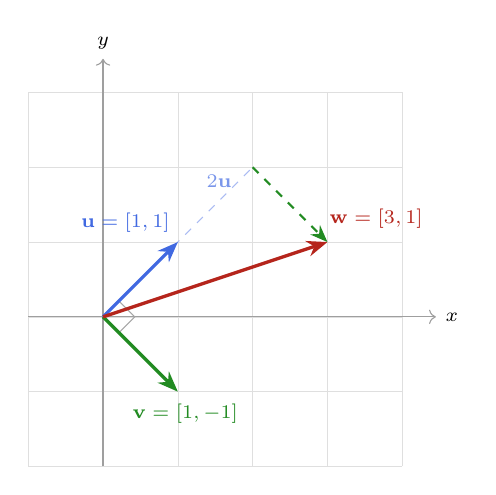
\begin{tikzpicture}[scale=0.95]
  \lattice{-1}{4}{-2}{3}
  \draw[gray!70] (0.212,0.212) -- (0.424,0) -- (0.212,-0.212);
  \draw[ForestGreen,dashed,thinarr] (2,2) -- (3,1);
  \draw[RoyalBlue!45,dashed] (0,0) -- (2,2);
  \draw[vecarr,RoyalBlue]   (0,0) -- (1,1);
  \draw[vecarr,ForestGreen] (0,0) -- (1,-1);
  \draw[vecarr,BrickRed]    (0,0) -- (3,1);
  \node[above left,font=\scriptsize,RoyalBlue]   at (1.02,1.0)  {$\vc{u}=[1,1]$};
  \node[below,font=\scriptsize,ForestGreen]      at (1.1,-1.04) {$\vc{v}=[1,-1]$};
  \node[above right,font=\scriptsize,BrickRed]   at (2.9,1.05)  {$\vc{w}=[3,1]$};
  \node[above,font=\scriptsize,RoyalBlue!70]     at (1.55,1.6)  {$2\vc{u}$};
\end{tikzpicture}
\end{center}

\begin{rmk}[Two is the most you can have]
In $\R^{2}$ there is no such thing as three mutually orthogonal nonzero vectors.
Suppose $\vc{u},\vc{v},\vc{w}$ were three of them. By the lemma
$\spanop\{\vc{u},\vc{v}\}=\R^{2}$, so $\vc{w}=\alpha\vc{u}+\beta\vc{v}$ for some
scalars. Dot that with $\vc{w}$ itself:
\[
  \norm{\vc{w}}^{2}
  = \langle\vc{w},\vc{w}\rangle
  = \alpha\langle\vc{w},\vc{u}\rangle + \beta\langle\vc{w},\vc{v}\rangle
  = 0 ,
\]
since $\vc{w}$ is orthogonal to both. So $\vc{w}=\vc{0}$, contradicting that it
was nonzero. The dimension of the space caps how many mutually orthogonal
directions it can hold --- at $2$ here, and at $n$ in $\R^{n}$.
\end{rmk}

%------------------------------------------------------------------------------
\subsection{The same principle in \texorpdfstring{$\R^{3}$}{R3}}
%------------------------------------------------------------------------------
Nothing in \S21.2 mentioned the number of coordinates. Run the identical
argument on three vectors: if $\vc{u},\vc{v},\vc{w}\in\R^{3}$ are nonzero and
mutually orthogonal, and
\[
  \alpha\vc{u} + \beta\vc{v} + \gamma\vc{w} = \vc{0} ,
\]
then dotting with $\vc{u}$ annihilates the $\beta$ and $\gamma$ terms and leaves
$\alpha\norm{\vc{u}}^{2}=0$, so $\alpha=0$. Dotting with $\vc{v}$ gives
$\beta=0$, and with $\vc{w}$ gives $\gamma=0$. So the three are linearly
independent, by exactly the same three lines.

\begin{ex}
The standard basis $\{\ivec,\jvec,\kvec\}$ of \S20.1 is mutually orthogonal and
each vector is nonzero, so it is independent --- which we had assumed rather
than checked. A less obvious triple:
\[
  \vc{u}=[\,1,\,2,\,2\,],\quad
  \vc{v}=[\,2,\,-2,\,1\,],\quad
  \vc{w}=[\,2,\,1,\,-2\,] ,
\]
where $\langle\vc{u},\vc{v}\rangle=2-4+2=0$,
$\langle\vc{u},\vc{w}\rangle=2+2-4=0$ and
$\langle\vc{v},\vc{w}\rangle=4-2-2=0$. All three have norm $3$. Mutually
orthogonal and nonzero, hence independent.
\end{ex}

\begin{rmk}[What is still owed]
Independence we have proved outright. To conclude that such a triple
\emph{spans} $\R^{3}$ we would need the $\R^{3}$ version of \S18.5 --- that any
three independent vectors in $\R^{3}$ span it --- and \S18.5 was proved only for
two vectors in $\R^{2}$, by an elimination that used the $2\times2$ quantity
$D=u_1v_2-u_2v_1$. The general statement, that $n$ independent vectors in
$\R^{n}$ form a basis, is true and we will prove it once we have the machinery
for $n\times n$ systems. Until then, treat the spanning half in $\R^{3}$ as
announced rather than established; the independence half is fully proved above
and is the part the rest of this section uses.
\end{rmk}

%------------------------------------------------------------------------------
\subsection{The converse fails}
%------------------------------------------------------------------------------
Orthogonality gives independence. The reverse implication does not hold, and one
example settles it.

\begin{ex}
Let $\vc{u}=[\,1,\,0\,]$ and $\vc{v}=[\,1,\,1\,]$. They are independent: no
scalar $\alpha$ satisfies $\alpha[1,0]=[1,1]$, since the second coordinate would
need $\alpha\cdot0=1$. But
\[
  \langle\vc{u},\vc{v}\rangle = 1(1)+0(1) = 1 \neq 0 ,
\]
so they are not orthogonal --- indeed
$\cos(\vc{u},\vc{v}) = 1/(1\cdot\sqrt2) = 1/\sqrt2$, an angle of $45^{\circ}$.
The basis $\{[1,2],[2,3]\}$ of \S18.1 is another: independent, but
$\langle[1,2],[2,3]\rangle = 2+6 = 8 \neq 0$.
\end{ex}

\noindent So the two conditions are not equivalent:
\[
  \text{mutually orthogonal (and nonzero)}
  \;\Longrightarrow\;
  \text{linearly independent},
\]
but not conversely. Orthogonality is the \emph{strictly stronger} condition, and
it is worth being precise about what the extra strength buys. Independence says
no vector is redundant --- none can be built from the others. Orthogonality says
something sharper: no vector has \emph{any} overlap with the others, not even a
partial one. In the language of \S12.4, the projection of one onto another is
the zero vector. Independent-but-not-orthogonal vectors do lean on each other
somewhat; they simply do not lean completely.

%------------------------------------------------------------------------------
\subsection{Why an orthogonal basis is worth having}
%------------------------------------------------------------------------------
Here is the practical payoff, and it is the reason orthogonality is pursued
rather than merely noticed.

Against a general basis $\{\vc{u},\vc{v}\}$, finding the coordinates of a vector
$\vc{w}$ means solving a linear system --- that was the work of \S18.1. Against
an \emph{orthogonal} basis, no system is needed. Write
$\vc{w}=\alpha\vc{u}+\beta\vc{v}$ and dot with $\vc{u}$; the $\beta$ term dies,
exactly as in \S21.2, leaving
\[
  \langle\vc{u},\vc{w}\rangle = \alpha\norm{\vc{u}}^{2},
  \qquad\text{so}\qquad
  \alpha = \frac{\langle\vc{u},\vc{w}\rangle}{\norm{\vc{u}}^{2}} ,
\]
and symmetrically $\beta=\langle\vc{v},\vc{w}\rangle/\norm{\vc{v}}^{2}$. Each
coordinate is computed \emph{independently of the other}, by one dot product and
one division.

Compare that expression with \S12.4: it is precisely the coefficient appearing
in $\proj{\vc{u}}{\vc{w}}$. So for an orthogonal basis,
\[
  \vc{w} = \proj{\vc{u}}{\vc{w}} + \proj{\vc{v}}{\vc{w}} ,
\]
a vector is the sum of its own shadows on the basis directions. This is the
general form of the remark in \S16.4 about why coordinates were free to read off
against $\{\ivec,\jvec\}$: that basis was orthogonal, and orthogonality was
doing the work all along --- being aligned with the axes was incidental.

\begin{ex}
Take the orthogonal basis $\vc{u}=[\,1,\,1\,]$, $\vc{v}=[\,1,\,-1\,]$ from
\S21.3 and the vector $\vc{w}=[\,3,\,1\,]$. Then $\norm{\vc{u}}^{2}=2$ and
$\norm{\vc{v}}^{2}=2$, so
\[
  \alpha = \frac{\langle\vc{u},\vc{w}\rangle}{2} = \frac{3+1}{2} = 2,
  \qquad
  \beta  = \frac{\langle\vc{v},\vc{w}\rangle}{2} = \frac{3-1}{2} = 1 .
\]
Checking: $2[\,1,\,1\,] + 1[\,1,\,-1\,] = [\,2,\,2\,]+[\,1,\,-1\,]
= [\,3,\,1\,]$. \checkmark\ No system was solved --- just two dot products,
which is the head-to-tail walk drawn in \S21.3.
\end{ex}

\lookahead If an orthogonal basis is this convenient, the obvious question is
whether one can always be manufactured: given any basis, can it be converted
into an orthogonal one spanning the same space? It can, and the procedure is
built out of exactly the piece we already have --- subtract off the projection,
as in \S12.6, so that what remains is orthogonal to what came before. Repeating
that step down a list of vectors is the Gram--Schmidt procedure.

%==============================================================================
\section{Subspaces as lines and planes}
%==============================================================================
With orthogonality settled, return to the subspaces of \S19. The classification
there was stated algebraically; it is worth saying what the answers look like.

%------------------------------------------------------------------------------
\subsection{In \texorpdfstring{$\R^{2}$}{R2}: lines}
%------------------------------------------------------------------------------
Section~19.4 found exactly three kinds of subspace of $\R^{2}$: the single point
$\{\vc{0}\}$, the whole plane, and everything in between --- which turned out to
be the lines through the origin. Two of those are degenerate: $\{\vc{0}\}$ has
dimension $0$ and $\R^{2}$ is not a proper subset. So the only interesting
subspace of the plane is a \textbf{line through the origin}, of dimension $1$,
and it is $\spanop\{\vc{u}\}$ for any nonzero $\vc{u}$ lying on it. That was the
line $L$ of \S18.6.

%------------------------------------------------------------------------------
\subsection{In \texorpdfstring{$\R^{3}$}{R3}: lines and planes}
%------------------------------------------------------------------------------
One dimension up, a new possibility appears. A subspace of $\R^{3}$ can be
spanned by \emph{two} independent vectors, and what they sweep out is a
\textbf{plane through the origin}, of dimension $2$.

We have already met one. The floor of \S20.2 is $\spanop\{\ivec,\jvec\}$: a
plane through the origin, a subspace of $\R^{3}$, with basis $\{\ivec,\jvec\}$
and dimension $2$. Nothing about it was special to the axes --- any two
independent vectors in $\R^{3}$ span a plane through the origin, tilted however
those two vectors happen to lie.

\begin{center}
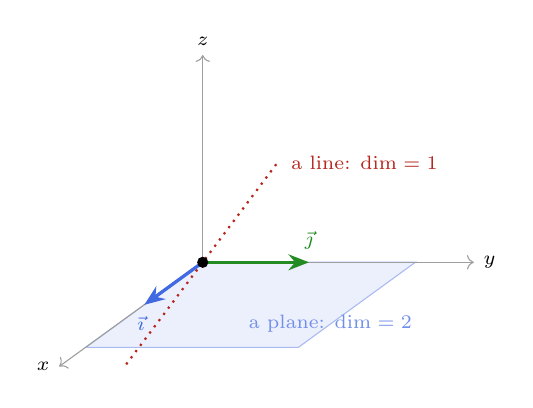
\begin{tikzpicture}[scale=1.35]
  \fill[RoyalBlue!10] (0,0) -- (-1.1,-0.8) -- (0.9,-0.8) -- (2,0) -- cycle;
  \draw[RoyalBlue!45] (0,0) -- (-1.1,-0.8) -- (0.9,-0.8) -- (2,0) -- cycle;
  \draw[axisline] (0,0) -- (-1.35,-0.98) node[left,font=\scriptsize,black]{$x$};
  \draw[axisline] (0,0) -- (2.55,0) node[right,font=\scriptsize,black]{$y$};
  \draw[axisline] (0,0) -- (0,1.95) node[above,font=\scriptsize,black]{$z$};
  \draw[BrickRed,dotted,thick] (-0.72,-0.96) -- (0.72,0.96);
  \draw[vecarr,RoyalBlue]   (0,0) -- (-0.55,-0.4);
  \draw[vecarr,ForestGreen] (0,0) -- (1,0);
  \fill (0,0) circle (1.5pt);
  \node[below,font=\scriptsize,RoyalBlue]   at (-0.58,-0.42) {$\ivec$};
  \node[above,font=\scriptsize,ForestGreen] at (1,0.03)      {$\jvec$};
  \node[font=\scriptsize,RoyalBlue!75]      at (1.2,-0.58)
        {a plane: $\dim=2$};
  \node[right,font=\scriptsize,BrickRed]    at (0.74,0.94)   {a line: $\dim=1$};
\end{tikzpicture}
\end{center}

\noindent So the picture to carry is:
\begin{center}
\renewcommand{\arraystretch}{1.35}
\begin{tabular}{@{}l l l@{}}
\toprule
\textbf{Dimension} & \textbf{Subspace of $\R^{2}$} & \textbf{Subspace of $\R^{3}$} \\
\midrule
$0$ & the origin            & the origin \\
$1$ & a line through origin & a line through the origin \\
$2$ & all of $\R^{2}$       & a plane through the origin \\
$3$ & ---                   & all of $\R^{3}$ \\
\bottomrule
\end{tabular}
\end{center}

\noindent Read across: the same dimension means the same kind of object; what
changes is whether that object exhausts the space it sits in. A plane is
everything in $\R^{2}$ and a thin slice of $\R^{3}$.

\begin{warn}
``Line'' and ``plane'' here always mean \emph{through the origin}. The line
$y=2x+1$ and the plane $z=1$ are not subspaces, for the reason given in \S19.3:
a subspace must contain $\vc{0}$, since scaling any of its elements by $0$
produces it. A line or plane that misses the origin is a perfectly good
geometric object, but it is not the span of anything and none of the machinery
of this unit applies to it.
\end{warn}

\lookahead The classification of subspaces of $\R^{3}$ --- origin, lines,
planes, everything --- is proved exactly as \S19.4 proved the $\R^{2}$ case:
take a nonzero vector, its span is already inside; if that is not everything,
take a vector outside it and enlarge; repeat. The only step not yet available is
the one flagged in \S21.4, that three independent vectors in $\R^{3}$ must span
it. Once that is in place, the argument runs unchanged, and it will keep running
in $\R^{n}$, where the subspaces are the origin, the lines, the planes, and so
on up through dimension $n$.

%==============================================================================
\section{The Pythagorean identity}
%==============================================================================
Orthogonality has one more consequence worth isolating, and it is the oldest
theorem in the subject wearing new clothes.

%------------------------------------------------------------------------------
\subsection{The setup}
%------------------------------------------------------------------------------
Let $\vc{u},\vc{v}\in\R^{2}$ be orthogonal, and consider their sum
$\vc{u}+\vc{v}$. Read it head to tail, as in \S7.1: walk along $\vc{u}$, then
along $\vc{v}$, and $\vc{u}+\vc{v}$ is the single arrow from start to finish.

That walk traces a triangle --- and this time the triangle has a right angle in
it, because the two legs are orthogonal. So the three side lengths are
$\norm{\vc{u}}$, $\norm{\vc{v}}$ and $\norm{\vc{u}+\vc{v}}$, with the sum as the
\emph{hypotenuse}, and Pythagoras predicts
\[
  \norm{\vc{u}}^{2} + \norm{\vc{v}}^{2} = \norm{\vc{u}+\vc{v}}^{2} .
\]

\begin{center}
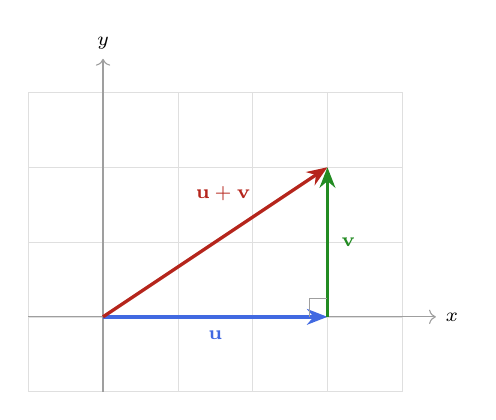
\begin{tikzpicture}[scale=0.95]
  \lattice{-1}{4}{-1}{3}
  \draw[vecarr,RoyalBlue]   (0,0) -- (3,0);
  \draw[vecarr,ForestGreen] (3,0) -- (3,2);
  \draw[vecarr,BrickRed]    (0,0) -- (3,2);
  \draw[gray!75] (2.76,0) -- (2.76,0.24) -- (3,0.24);
  \node[below,font=\scriptsize,RoyalBlue]      at (1.5,-0.06) {$\vc{u}$};
  \node[right,font=\scriptsize,ForestGreen]    at (3.06,1.0)  {$\vc{v}$};
  \node[above left,font=\scriptsize,BrickRed]  at (2.1,1.42)  {$\vc{u}+\vc{v}$};
\end{tikzpicture}
\end{center}

\noindent Note that this is a genuine right triangle only because
$\langle\vc{u},\vc{v}\rangle=0$. For a general pair the head-to-tail triangle of
\S7.2 has no right angle and the identity is false --- which is exactly why the
triangle inequality there was an \emph{inequality}.

%------------------------------------------------------------------------------
\subsection{The proof}
%------------------------------------------------------------------------------
Before proving it, recall the two collections of algebraic facts the computation
will use. Vector addition and scalar multiplication obey the laws collected in
\S8.4 --- commutativity, associativity, distributivity and the rest. The dot
product obeys the laws collected in \S11.8: it is symmetric, it distributes over
addition, scalars pull out of it, and $\langle\vc{w},\vc{w}\rangle=\norm{\vc{w}}^{2}$.
With those in hand the proof is four lines.

Start from the identity $\norm{\vc{w}}^{2}=\langle\vc{w},\vc{w}\rangle$ of
\S11.6, applied to $\vc{w}=\vc{u}+\vc{v}$, and expand by distributing twice:
\begin{align*}
  \norm{\vc{u}+\vc{v}}^{2}
   &= \bigl\langle \vc{u}+\vc{v},\ \vc{u}+\vc{v} \bigr\rangle \\[2pt]
   &= \langle\vc{u},\vc{u}\rangle + \langle\vc{u},\vc{v}\rangle
      + \langle\vc{v},\vc{u}\rangle + \langle\vc{v},\vc{v}\rangle \\[2pt]
   &= \norm{\vc{u}}^{2} + 2\langle\vc{u},\vc{v}\rangle + \norm{\vc{v}}^{2} ,
\end{align*}
where the last step used symmetry, $\langle\vc{u},\vc{v}\rangle
=\langle\vc{v},\vc{u}\rangle$, to combine the two middle terms. Now impose the
hypothesis. Orthogonality says $\langle\vc{u},\vc{v}\rangle=0$, so the middle
term vanishes and
\[
  \boxed{\;\norm{\vc{u}+\vc{v}}^{2} = \norm{\vc{u}}^{2} + \norm{\vc{v}}^{2}\;}
\]
which is the identity. \hfill$\blacksquare$

\begin{rmk}[Nothing here is new except the cancellation]
The expansion
$\norm{\vc{u}+\vc{v}}^{2}=\norm{\vc{u}}^{2}+2\langle\vc{u},\vc{v}\rangle+\norm{\vc{v}}^{2}$
is not new --- it is the computation already used at the end of \S13 to derive
the triangle inequality from Cauchy--Schwarz. It holds for \emph{every} pair of
vectors. The Pythagorean identity is that general expansion in the one case
where the cross term $2\langle\vc{u},\vc{v}\rangle$ happens to be zero. So
Pythagoras is not a separate theorem about right triangles; it is the special
case of an algebraic identity, and the right angle is what kills the middle
term.
\end{rmk}

\begin{rmk}[It runs both ways]
The expansion also gives the converse for free. If
$\norm{\vc{u}+\vc{v}}^{2}=\norm{\vc{u}}^{2}+\norm{\vc{v}}^{2}$, then comparing
with the general expansion forces $2\langle\vc{u},\vc{v}\rangle=0$, hence
$\langle\vc{u},\vc{v}\rangle=0$, hence $\vc{u}$ and $\vc{v}$ are orthogonal. So
\[
  \vc{u}\perp\vc{v}
  \qquad\Longleftrightarrow\qquad
  \norm{\vc{u}+\vc{v}}^{2}=\norm{\vc{u}}^{2}+\norm{\vc{v}}^{2} ,
\]
and the Pythagorean identity is not merely a consequence of orthogonality but a
\emph{characterisation} of it --- one more entry alongside
$\langle\vc{u},\vc{v}\rangle=0$ and $\theta=\pi/2$.
\end{rmk}

\begin{ex}
Take $\vc{u}=[\,3,\,0\,]$ and $\vc{v}=[\,0,\,4\,]$, which are orthogonal since
$\langle\vc{u},\vc{v}\rangle=0$. Then $\vc{u}+\vc{v}=[\,3,\,4\,]$ and
\[
  \norm{\vc{u}}^{2}+\norm{\vc{v}}^{2} = 9+16 = 25 = \norm{[\,3,\,4\,]}^{2} .
\]
The $3$--$4$--$5$ triangle, recovered from the dot product.

For a pair not aligned with the axes, take $\vc{u}=[\,1,\,1\,]$ and
$\vc{v}=[\,1,\,-1\,]$ from \S21.3. Then $\vc{u}+\vc{v}=[\,2,\,0\,]$ and
$2+2=4$. \checkmark
\end{ex}

%------------------------------------------------------------------------------
\subsection{In \texorpdfstring{$\R^{3}$}{R3} and beyond}
%------------------------------------------------------------------------------
The proof never mentioned coordinates, so it transfers untouched. For orthogonal
$\vc{u},\vc{v}\in\R^{3}$ the same four lines give
$\norm{\vc{u}+\vc{v}}^{2}=\norm{\vc{u}}^{2}+\norm{\vc{v}}^{2}$.

\begin{ex}
From \S21.4, $\vc{u}=[\,1,\,2,\,2\,]$ and $\vc{v}=[\,2,\,-2,\,1\,]$ are
orthogonal with $\norm{\vc{u}}=\norm{\vc{v}}=3$. Their sum is
$[\,3,\,0,\,3\,]$, and
\[
  \norm{\vc{u}+\vc{v}}^{2} = 9+0+9 = 18 = 9 + 9
  = \norm{\vc{u}}^{2}+\norm{\vc{v}}^{2} . \quad\checkmark
\]
\end{ex}

\noindent The moral is worth stating in one line: lengths do not add, but
\emph{squared} lengths do --- provided the two directions are orthogonal.

%------------------------------------------------------------------------------
\subsection{An exact accounting of a projection}
%------------------------------------------------------------------------------
The identity earns its keep immediately, because \S12.6 built an orthogonal pair
for us. Recall that any $\vc{v}$ splits as
\[
  \vc{v} = \underbrace{\proj{\vc{u}}{\vc{v}}}_{\text{along }\vc{u}}
         + \underbrace{\bigl(\vc{v}-\proj{\vc{u}}{\vc{v}}\bigr)}_{\perp\,\vc{u}} ,
\]
and that the second piece is orthogonal to $\vc{u}$ --- hence orthogonal to the
first piece, which is a multiple of $\vc{u}$. Two orthogonal vectors summing to
$\vc{v}$: exactly the hypothesis of \S23.2. So
\[
  \norm{\vc{v}}^{2}
  = \norm{\proj{\vc{u}}{\vc{v}}}^{2}
    + \norm{\vc{v}-\proj{\vc{u}}{\vc{v}}}^{2} .
\]

\noindent Read that as a budget. The squared length of $\vc{v}$ divides exactly
into the part explained by $\vc{u}$ and the part left over, with nothing
unaccounted for.

\begin{rmk}[Cauchy--Schwarz, one more time]
This sharpens \S13. There we argued that a shadow is never longer than the
object casting it, $\lvert\comp{\vc{u}}{\vc{v}}\rvert\le\norm{\vc{v}}$, and
turned it into Cauchy--Schwarz. The budget above proves the same inequality and
says precisely what the slack is: since
$\norm{\proj{\vc{u}}{\vc{v}}}=\lvert\comp{\vc{u}}{\vc{v}}\rvert$, we get
\[
  \norm{\vc{v}}^{2} - \comp{\vc{u}}{\vc{v}}^{2}
  = \norm{\vc{v}-\proj{\vc{u}}{\vc{v}}}^{2} \;\ge\; 0 ,
\]
so the shadow falls short of the object by exactly the squared length of the
orthogonal remainder --- and equality holds precisely when that remainder is
$\vc{0}$, which is when $\vc{v}$ already lies along $\vc{u}$. That is the
equality case of Cauchy--Schwarz, recovered with the gap measured rather than
merely bounded.
\end{rmk}

\lookahead Squared lengths adding over orthogonal pieces is the reason
orthogonal decompositions are the workhorse of applied linear algebra. Split a
vector into mutually orthogonal components and its squared length distributes
across them without interference, so each component's contribution can be
measured, ranked, and discarded independently of the others. That is the
principle behind least squares, behind Parseval's identity in signal
processing, and behind deciding how many components of a decomposition are worth
keeping.

%==============================================================================
\section{Generalizing to \texorpdfstring{$\R^{n}$}{Rn}}
%==============================================================================
We began this unit with arrows in a plane and have twice widened the setting ---
to $\R^{3}$ in \S20, and to a whole family of norms in \S14 --- without the
definitions objecting. It is time to stop widening one dimension at a time.

Fix a natural number $n$ and work in $\R^{n}$. Everything built so far
generalizes, and this section collects the generalizations in one place. Each
formula reduces to the one you already know when $n=2$ or $n=3$; the only real
change is notational, since writing out $n$ terms is impossible and we use the
$\Sigma$ notation of Lecture~0 instead.

%------------------------------------------------------------------------------
\subsection{The space and its standard basis}
%------------------------------------------------------------------------------
\begin{defn}[$\R^{n}$]
For a natural number $n$,
\[
  \R^{n}
  \;=\;
  \bigl\{\,(x_1,x_2,\dots,x_n) \;\bigm|\; x_i\in\R \text{ for } i=1,\dots,n \,\bigr\},
\]
the set of ordered $n$-tuples of real numbers. We write a vector as
$\vc{v}=[\,v_1,\,v_2,\,\dots,\,v_n\,]$ and call $v_i$ its $i$-th
\textbf{coordinate}.
\end{defn}

\noindent The standard basis needs $n$ vectors, and the letters $\ivec,\jvec,\kvec$
run out at three. So they are renamed and indexed:
\[
  \vc{e}_1 = [\,1,0,0,\dots,0\,],\quad
  \vc{e}_2 = [\,0,1,0,\dots,0\,],\quad\dots,\quad
  \vc{e}_n = [\,0,0,\dots,0,1\,] ,
\]
where $\vc{e}_i$ carries a $1$ in slot $i$ and $0$ everywhere else. In $\R^{3}$
these are exactly $\ivec,\jvec,\kvec$ under new names.

They are orthonormal for the same reason as before: $\norm{\vc{e}_i}=1$, and for
$i\neq j$ the product $\langle\vc{e}_i,\vc{e}_j\rangle$ has a zero in every term.
Every vector expands over them,
\[
  \vc{v} = \sum_{i=1}^{n} v_i\,\vc{e}_i ,
\]
and by \S21.6 the coordinates are read off by projection, $v_i=\langle\vc{e}_i,\vc{v}\rangle$,
with no system to solve. Since a basis has $n$ vectors,
\[
  \dim\R^{n}=n .
\]

%------------------------------------------------------------------------------
\subsection{Every definition, in \texorpdfstring{$n$}{n} dimensions}
%------------------------------------------------------------------------------
Here is the whole unit, restated. In each row $\vc{u},\vc{v},\vc{x},\vc{y}\in\R^{n}$
and $\alpha\in\R$, and every sum runs from $i=1$ to $n$.

\begin{center}
\renewcommand{\arraystretch}{2.0}
\begin{tabular}{@{}l l l@{}}
\toprule
\textbf{Object} & \textbf{Where} & \textbf{Definition in $\R^{n}$} \\
\midrule
Addition & \S7
  & $\vc{u}+\vc{v} = [\,u_1+v_1,\ \dots,\ u_n+v_n\,]$ \\
Subtraction & \S7
  & $\vc{u}-\vc{v} = [\,u_1-v_1,\ \dots,\ u_n-v_n\,]$ \\
Scalar multiplication & \S8
  & $\alpha\vc{v} = [\,\alpha v_1,\ \dots,\ \alpha v_n\,]$ \\
Dot product & \S11.3
  & $\displaystyle\langle\vc{u},\vc{v}\rangle=\sum_{i=1}^{n}u_iv_i$ \\
Euclidean norm & \S2
  & $\displaystyle\norm{\vc{v}}=\sqrt{\sum_{i=1}^{n}v_i^{2}}=\sqrt{\langle\vc{v},\vc{v}\rangle}$ \\
$p$-norm & \S14.6
  & $\displaystyle\norm{\vc{v}}_p=\Bigl(\sum_{i=1}^{n}\lvert v_i\rvert^{p}\Bigr)^{1/p}$ \\
$\infty$-norm & \S14.7
  & $\displaystyle\norm{\vc{v}}_\infty=\max_{1\le i\le n}\lvert v_i\rvert$ \\
Metric & \S14.2
  & $\displaystyle d(\vc{x},\vc{y})=\norm{\vc{x}-\vc{y}}=\sqrt{\sum_{i=1}^{n}(x_i-y_i)^{2}}$ \\
Cosine similarity & \S11.4
  & $\displaystyle\cos(\vc{u},\vc{v})=\frac{\langle\vc{u},\vc{v}\rangle}{\norm{\vc{u}}\,\norm{\vc{v}}}$ \\
Orthogonality & \S11.7
  & $\vc{u}\perp\vc{v} \iff \langle\vc{u},\vc{v}\rangle=0$ \\
Component & \S12.4
  & $\displaystyle\comp{\vc{u}}{\vc{v}}=\frac{\langle\vc{u},\vc{v}\rangle}{\norm{\vc{u}}}$ \\
Projection & \S12.4
  & $\displaystyle\proj{\vc{u}}{\vc{v}}=\frac{\langle\vc{u},\vc{v}\rangle}{\norm{\vc{u}}^{2}}\,\vc{u}$ \\
\bottomrule
\end{tabular}
\end{center}

\noindent And the structural notions, for a collection
$\vc{u}_1,\dots,\vc{u}_k\in\R^{n}$:

\begin{center}
\renewcommand{\arraystretch}{2.0}
\begin{tabular}{@{}l l l@{}}
\toprule
\textbf{Object} & \textbf{Where} & \textbf{Definition in $\R^{n}$} \\
\midrule
Linear combination & \S16.2
  & $\displaystyle\sum_{i=1}^{k}\alpha_i\vc{u}_i$, \quad $\alpha_i\in\R$ \\
Span & \S16.3
  & $\displaystyle\spanop\{\vc{u}_1,\dots,\vc{u}_k\}
     = \Bigl\{\sum_{i=1}^{k}\alpha_i\vc{u}_i \;\Bigm|\; \alpha_i\in\R\Bigr\}$ \\
Linear independence & \S18.4
  & $\displaystyle\sum_{i=1}^{k}\alpha_i\vc{u}_i=\vc{0}
     \ \Longrightarrow\ \alpha_1=\cdots=\alpha_k=0$ \\
Linear dependence & \S18.4
  & some $\alpha_i$ not all zero give $\displaystyle\sum_{i=1}^{k}\alpha_i\vc{u}_i=\vc{0}$ \\
Basis & \S16.3
  & spans, and is linearly independent \\
Dimension & \S17
  & the number of vectors in a basis \\
Subspace & \S19.3
  & non-empty $S\subseteq\R^{n}$ closed under $+$ and scalar multiplication \\
\bottomrule
\end{tabular}
\end{center}

\begin{rmk}
Notice how little the $\Sigma$ notation is doing beyond bookkeeping. The dot
product in $\R^{2}$ was $u_1v_1+u_2v_2$ and in $\R^{3}$ was
$u_1v_1+u_2v_2+u_3v_3$; the notation $\sum_{i=1}^{n}u_iv_i$ says ``keep going''
and nothing more. Definitions that were already written without reference to
coordinates --- cosine similarity, the projection, the metric --- did not change
at all, exactly as the table in \S20.3 predicted.
\end{rmk}

%------------------------------------------------------------------------------
\subsection{The laws and identities that come with them}
%------------------------------------------------------------------------------
Every algebraic fact in the unit was proved either componentwise, in which case
the proof runs over $n$ slots instead of $2$, or from the laws, in which case it
never mentioned coordinates at all. Either way it survives:

\begin{itemize}[leftmargin=1.4em,itemsep=4pt]
  \item the eight laws of vector arithmetic, \textbf{A1}--\textbf{A4} and
        \textbf{S1}--\textbf{S4} (\S8.4);
  \item the dot-product laws \textbf{D1}--\textbf{D4} and bilinearity
        (\S11.8), including
        $\langle\vc{u},\vc{u}\rangle=\norm{\vc{u}}^{2}$;
  \item the norm axioms \textbf{N1}--\textbf{N3} (\S15.1), and Minkowski's
        inequality for every $p\ge1$;
  \item the metric axioms \textbf{M1}--\textbf{M4} (\S14.1);
  \item \textbf{Cauchy--Schwarz}, $\lvert\langle\vc{u},\vc{v}\rangle\rvert
        \le\norm{\vc{u}}\norm{\vc{v}}$ (\S13), and H\"older with conjugate
        exponents (\S15.3);
  \item the \textbf{triangle inequality}
        $\norm{\vc{u}+\vc{v}}\le\norm{\vc{u}}+\norm{\vc{v}}$ (\S7.2);
  \item the expansion
        $\norm{\vc{u}+\vc{v}}^{2}
         =\norm{\vc{u}}^{2}+2\langle\vc{u},\vc{v}\rangle+\norm{\vc{v}}^{2}$,
        and with it the \textbf{Pythagorean identity} (\S23): if
        $\langle\vc{u},\vc{v}\rangle=0$ then
        $\norm{\vc{u}+\vc{v}}^{2}=\norm{\vc{u}}^{2}+\norm{\vc{v}}^{2}$;
  \item the \textbf{orthogonal decomposition}
        $\vc{v}=\proj{\vc{u}}{\vc{v}}+\bigl(\vc{v}-\proj{\vc{u}}{\vc{v}}\bigr)$
        (\S12.6), with the two pieces orthogonal;
  \item \textbf{orthogonal $\Rightarrow$ independent} for nonzero vectors
        (\S21.2), by the same proof: dot with $\vc{u}_j$, every cross term dies,
        and $\alpha_j\norm{\vc{u}_j}^{2}=0$ forces $\alpha_j=0$.
\end{itemize}

\noindent The counting statements adjust in the obvious way: a basis for
$\R^{n}$ has $n$ vectors, at most $n$ vectors in $\R^{n}$ can be mutually
orthogonal and nonzero, and the subspaces of $\R^{n}$ are the origin, the lines
through it, the planes through it, and so on up to $\R^{n}$ itself --- of every
dimension from $0$ to $n$.

%------------------------------------------------------------------------------
\subsection{An example you cannot draw}
%------------------------------------------------------------------------------
\begin{ex}
Work in $\R^{4}$ with
\[
  \vc{u} = [\,1,\,1,\,1,\,1\,],
  \qquad
  \vc{v} = [\,1,\,1,\,-1,\,-1\,] .
\]
Norms: $\norm{\vc{u}}=\sqrt{1+1+1+1}=2$, and likewise $\norm{\vc{v}}=2$. The
other members of the family: $\norm{\vc{u}}_1=4$, $\norm{\vc{u}}_2=2$,
$\norm{\vc{u}}_\infty=1$, so $1\le2\le4$, the ordering of \S14.8.

Dot product: $\langle\vc{u},\vc{v}\rangle = 1+1-1-1 = 0$, so $\vc{u}$ and
$\vc{v}$ are orthogonal --- and by \S21.2 independent --- although no picture
was consulted and none is available.

Pythagoras: $\vc{u}+\vc{v}=[\,2,\,2,\,0,\,0\,]$, so
$\norm{\vc{u}+\vc{v}}^{2}=4+4=8$, and $\norm{\vc{u}}^{2}+\norm{\vc{v}}^{2}=4+4=8$.
\checkmark

Distance: $\vc{u}-\vc{v}=[\,0,\,0,\,2,\,2\,]$, so $d(\vc{u},\vc{v})=\sqrt{8}=2\sqrt2$,
while $d_1=4$ and $d_\infty=2$.
\end{ex}

\begin{ex}
Adjoin two more vectors to the pair above:
\[
  \vc{w} = [\,1,\,-1,\,1,\,-1\,],
  \qquad
  \vc{z} = [\,1,\,-1,\,-1,\,1\,] .
\]
Every one of the six pairings has dot product zero --- for instance
$\langle\vc{u},\vc{w}\rangle = 1-1+1-1 = 0$ and
$\langle\vc{v},\vc{z}\rangle = 1-1+1-1 = 0$. So $\{\vc{u},\vc{v},\vc{w},\vc{z}\}$
is a set of four mutually orthogonal nonzero vectors in $\R^{4}$, hence
independent, hence a basis. Coordinates against it cost four dot products and
four divisions by $4$, with no system solved. Try to visualise it and you will
fail; the arithmetic does not care.
\end{ex}

%------------------------------------------------------------------------------
\subsection{What is lost, and what is not}
%------------------------------------------------------------------------------
One thing genuinely does not survive: the picture. In $\R^{2}$ and $\R^{3}$ you
can see the angle between two vectors and check a claim by drawing it. In
$\R^{4}$ and beyond you cannot, and this is the situation flagged twice already
--- in the remark of \S15.3 and again in \S20.4.

The resolution is to reverse the order of definition. In the plane we defined
$\theta$ geometrically in \S10.3 and \emph{derived}
$\cos(\vc{u},\vc{v})=\langle\vc{u},\vc{v}\rangle/(\norm{\vc{u}}\norm{\vc{v}})$
from the law of cosines. In $\R^{n}$ there is no geometric $\theta$ to start
from, so the quotient becomes the definition:
\[
  \theta := \arccos\!\left(
    \frac{\langle\vc{u},\vc{v}\rangle}{\norm{\vc{u}}\,\norm{\vc{v}}}\right)
  \in [\,0,\pi\,] .
\]
That this is legitimate is exactly what Cauchy--Schwarz provides: it guarantees
the quotient lies in $[-1,1]$, which is the domain of $\arccos$. Without the
inequality, the definition would be writing nonsense. This is why \S15.3
insisted that Cauchy--Schwarz is a statement about inner products rather than a
fact about triangles --- the triangle was scaffolding, and here the scaffolding
is gone while the statement remains.

\begin{rmk}[One operation that does not generalize]
The cross product of \S20.4 is genuinely special to $\R^{3}$. It takes two
vectors and returns a third perpendicular to both, and no such operation exists
in $\R^{2}$ or in $\R^{4}$. When we need ``the directions orthogonal to a given
set'' in general dimensions, we will get them from the dot product instead, by
solving $\langle\vc{u},\vc{x}\rangle=0$ --- a linear system.
\end{rmk}

\lookahead With $\R^{n}$ in place the unit has done its job. Every object from
here on --- a system of equations, a matrix, an eigenvector, a least-squares fit
--- lives in some $\R^{n}$, and the norms, dot products, projections and
orthogonality of this unit are the tools used on all of them. What we lack is a
way to describe transformations \emph{between} such spaces, and a systematic
method for the linear systems that keep appearing whenever a basis is not
orthogonal. Both are matrices, and they are next.

\end{document}
